\documentclass[a4paper,12pt]{article}

\usepackage{amsmath,amssymb,multicol,tikz,enumitem}
\usepackage[margin=2cm]{geometry}
%\usetikzlibrary{calc}
\usepackage{amsmath}
\usepackage{amsthm}
\usepackage{thmtools}
\usepackage{hyperref}
\usepackage{enumerate}
\usepackage{xcolor}

\pagestyle{empty}

\newcommand\Q{\mathbf{Q}}
\newcommand\R{\mathbf{R}}
\newcommand\Z{\mathbf{Z}}

\newcommand\answer[1]{}
\newcommand\ans[1]{}
%\newcommand\answer[1]{\\[5pt]{\color{blue}{#1}}\hfill{\color{blue}}\\[-5pt]} 
%\newcommand\ans[1]{{\color{blue}{#1}}}

\usepackage{array}
\newcolumntype{P}[1]{>{\centering\arraybackslash}p{#1}}

\newcommand\indd{${}$\hspace{20pt}}

\declaretheoremstyle[headfont=\normalfont\bfseries,notefont=\mdseries\bfseries,bodyfont = \normalfont,headpunct={:}]{normalhead}
\declaretheorem[name={Uzdevums}, style=normalhead,numberwithin=section]{problem}

\setcounter{section}{02}

\setlength\parindent{0pt}

\renewcommand{\figurename}{Attēls}

\begin{document}

\begin{center}
\parbox{3.5cm}{\flushleft\bf Modulārā aritmētika} \hfill {\bf\LARGE Sacensības 2021\#02} \hfill \parbox{3.5cm}{\flushright\bf 2021-03-04} \\[2pt]
{\rm\footnotesize Par šo LU NMS atbalstīto pasākumu\\ atbild {\tt kalvis.apsitis@gmail.com}.}
\end{center}

%\hrule\vspace{2pt}\hrule
\hrule




\vspace{10pt}
\begin{problem}
Regulārā $360$-stūrī virsotnes apzīmētas ar veseliem skaitļiem no $0$ līdz $359$. 
\begin{itemize}
\item Ar ziliem nogriežņiem savienotas virsotnes $a,b$, kurām $a+b \equiv 37 \pmod{360}$. 
\item Ar sarkaniem nogriežņiem savienotas virsotnes $a,b$, kurām $a+b \equiv 151 \pmod{360}$. 
\end{itemize}
Atrast mazāko leņķi (grādos) kuru var veidot zils nogrieznis ar sarkanu nogriezni. 
(Ja krustojoties veidojas divi leņķi $x$ un $180^{\circ}-x$, ierakstīt mazāko pozitīvo $x$ vērtību.)
\answer{

{\bf Atbilde.} $\mathtt{57}$.

Apzīmējam virsotnes ar $A_0,A_1,\ldots,A_{359}$. 
Visi zilie nogriežņi ir paralēli nogrieznim $A_{0}A_{37}$, jo $0+37 \equiv 37 \pmod{360}$. Pārceļot šo 
nogriezni paralēli, summas atlikums, dalot ar $360$ nemainās.

Savukārt visi sarkanie nogriežņi ir paralēli nogrieznim 
$A_{37}A_{114}$, jo $37 + 114 \equiv 151 \pmod{360}$) un visi citi sarkanie nogriežņi ir tam paralēli.

Leņķis $\sphericalangle A_0A_{37}A_{114}$ balstās uz riņķa loka $A_0A_{114}$ garākās daļas, kas lielāka par $180^{\circ}$. 
Šis loks ir $360^{\circ} - 114^{\circ} = 246^{\circ}$, tāpēc $\sphericalangle A_0A_{37}A_{114}$ ir puse no tā: $123^{\circ}$. 
Bet tā kā šis leņķis ir plats un jāieraksta mazākā vērtība, ko veido divi krustiski nogriežņi, 
tad mazākais leņķis starp zilu un sarkanu nogriezni ir $180^{\circ} - 123^{\circ} = 57^{\circ}$.
}
\end{problem}



\vspace{20pt}
\begin{problem}
Ar kādu periodu mainās pēdējie $10$ cipari skaitļa $5^n$ decimālpierakstā? 
(Var pieņemt, ka $n$ vērtība ir pietiekami liela un priekšperiods jau ir beidzies.)
\answer{

{\bf Atbilde.} $\mathtt{256}$\\
Pamatosim, ka skaitļa $5$ pakāpēm pēdējie $k$ cipari (ja $k >2$) mainās periodiski ar periodu 
$2^{k-2}$. 


\vspace{5pt}
{\bf Apgalvojums 1.} Apskatām atlikumus pēc moduļa $2^k$, kas ir divnieka pakāpe, un $a$ ir nepāra skaitlis. 
Jebkuram veselam $k \geq 3$ un jebkuram $a \equiv 1 \pmod{2}$ izpildās šāda sakarība:
\[ a^{2^{k-2}} \equiv 1 \pmod{2^k} \]
(Šis apgalvojums nozīmē, ka skaitļiem $2^k = 8,16,32,\ldots$ Eilera teorēmas paredzētā atgriešanās pie atlikuma $1$
\[ a^{\varphi(2^k)} \equiv 1 \pmod{2^k} \]
faktiski iestājas divreiz ātrāk nekā paredz Eilera teorēma, jo $\varphi(2^k) = 2^{k-1}$, bet 
atgriešanās pie atlikuma $1$ jau kāpinot skaitli $a$ pakāpē $2^{k-2}$. 

\vspace{5pt}
{\bf Bāze.} Ja $k=3$, tad iespējamas četras nepāra kongruenču klases $a = 1,3,5,7$. 
Ikvienu no tām kāpinot pakāpē $2^{k-2} = 2^1 =2$ iegūsim 
\[ 1^2 \equiv 3^2 \equiv 5^2 \equiv 7^2 \equiv 1 \pmod{8}. \]

\vspace{5pt}
{\bf Induktīvā pāreja.} Pieņemsim, ka ir vērtība $k=m$, kurai Apgalvojums 1 izpildās. 
Faktiski tas nozīmē, ka virknē $a^1, \ldots, a^{2^{m-2}}$ ir ne vairāk kā $2^{m-2}$
dažādi atlikumi, dalot ar $2^m$ (kaut arī nepāra skaitļu no $1$ līdz $2^{m}$ ir 
tieši $2^{m-1}$). Apzīmēsim šos atlikumus ar $r_1,r_2,\ldots,r_{2^{m-2}}$ (visi tie ir 
kongruenču klases $\pmod{2^m}$)

Tad nākamajai vērtībai $k=m+1$ varam dabūt divreiz vairāk atlikumu, jo 
\[r_1 \equiv r_1 + 2^m \pmod{2^m},\;\;\text{bet}\ r_1 \not\equiv r_1 + 2^m \pmod{2^{m+1}}. \]
T.i. katra no kongruenču klasēm pēc moduļa $2^m$ ``sašķeļas uz pusēm'', no tās rodas divas
kongruenču klases pēc moduļa $2^{m+1}$. Tāpēc lielākais iespējamais dažādo atlikumu skaits 
starp skaitļa $a$ pakāpēm $\pmod{2^{m+1}}$ būs $2^{m-1}$.

Pēc Eilera teorēmas $a^{2^m} \equiv 1 \pmod{2^{m+1}}$, tāpēc mazākais veselais skaitlis $x>1$, 
kuram $a^x \equiv 1 \pmod{2^{m+1}}$ būs skaitļa $2^m$ dalītājs (tātad $x$ arī ir divnieka pakāpe). 
Pēc induktīvā pieņēmuma (un kongruenču klašu sašķelšanās uz pusēm) redzam, ka $x \leq 2^{m-1}$. 
Tātad $x$ ir tāda divnieka pakāpe kas ir mazāka par $2^m$ un tātad ir arī skaitļa $2^{m-1}$ dalītājs. 
Esam ieguvuši, ka 
\[ a^{2^{m-1}} \equiv 1 \pmod{2^{m+1}}, \]
kas pabeidz induktīvo pāreju. $\blacksquare$


\vspace{10pt}
{\bf Apgalvojums 2.} Mazākais $x>1$, kuram $5^x \equiv 1 \pmod{2^k}$ ir precīzi 
vienāds ar $2^{k-2}$. 

\vspace{5pt} 
No Apgalvojuma 1 seko, ka $x \leq 2^{k-2}$. 
Kāpēc $x$ nevar būt mazāks par $2^{k-2}$ arī var pierādīt ar indukciju, ja sadala reizinātājos: 
\[ 5^{k-2} - 1 = \left( 5^{k-3} - 1 \right)\left( 5^{k-3} + 1 \right). \]
Un ievērojam, ka otrais reizinātājs dalās ar $2$, bet ne ar $4$. 
Sk. detalizētāk \url{https://bit.ly/3v79bm1}.  $\blacksquare$


\vspace{10pt}
{\bf Apgalvojums 3.} Skaitļu $5^n$ pēdējie $k$ cipari mainās ar periodu $2^{k-2}$, ja
$n$ vērtība ir pietiekami liela (ja $n \geq k$). 

\vspace{5pt} 
Lai šo apgalvojumu pamatotu, uzrakstām kongruences ar $5^n$ vērtībām pēc moduļa $10^k$; 
tad saīsinām visas šīs kongruences ar reizinātāju $5^k$ un atsaucamies uz Apgalvojumu 2, 
lai pamatotu, ka cikls iestājas tieši pēc $2^{k-2}$ soļiem. $\blacksquare$

Apgalvojums 3 nozīmē to, ka pēdējie $10$ cipari mainās ar periodu $2^8 = 256$, kas arī 
pamato mūsu atbildi. 
}
\end{problem}



\vspace{20pt}
\begin{problem}
$F(0)=0$; $F(1)=1$; $F(k+2) = F(k+1) + F(k)$ ir Fibonači skaitļu virkne.
Atrast mazāko veselo pozitīvo skaitli $n$, kuram Fibonači skaitlis $F(n)$ dod atlikumu $5$, 
dalot ar $8$ un vienlaikus arī atlikumu $13$, dalot ar $21$. 
\answer{

{\bf Atbilde.} $\mathtt{7}$\\
Varam atrast, ka $F(7) = 13$, kas dod abus vajadzīgos atlikumus. 

Šīm konkrētajām vērtībām bija visai viegli uzminēt atrisinājumu kongruenču sistēmai. 
Var viegli formulēt arī drusku sarežģītākus piemērus. Piemēram, atrast mazāko $n$, kuram $F(n)$ apmierina kongruences:
\[ \left\{ \begin{array}{l}
F(n) \equiv 0 \pmod{10}\\
F(n) \equiv 0 \pmod{13}\\
\end{array} \right. \]
Var pamatot, ka ar $10$ dalās visi tie $F(n)$, kuriem $n$ dalās ar $15$, bet ar $13$ dalās visi tie $F(n)$, kuriem 
$n$ dalās ar $7$. Tāpēc mazākais pozitīvais $n$, kuram $F(n)$ dalās ar $130$ būs $15 \cdot 7 = 105$. 
}
\end{problem}


\vspace{20pt}
\begin{problem}
Ar cik daudzām nullēm beidzas skaitļa $11^{10^{1918}}-1$ decimālpieraksts?
\answer{

{\bf Atbilde.} $\mathtt{1919}$.\\

Lietojam {\em Kāpinātāja pacelšanas lemmu} - sk. \url{https://bit.ly/38orQjt}.
$x = 11$ un $y=1$, kāpinātājs ir $n=10^{1918}$.
Izvēlamies divas pirmskaitļu vērtības: $p=2$ un $p=5$. Izmantosim kāpinātāja
pacelšanas lemmas abus gadījumus (tas atšķiras nepāra pirmskaitlim $p=5$ un 
vienīgajam pāra pirmskaitlim $p=2$). 

\[ \nu_5\left( x^n - y^n \right) = \nu_5(x - y) + \nu_5(n) = \nu_5(11-1) + \nu_5(10^{1918}) = 1 + 1918 = 1919. \]
\[ \nu_2\left( x^n - y^n \right) = \nu_2(x - y) + \nu_2(n) + \nu_2(x + y) - 1 = \nu_2(10) + \nu_2(10^{1918}) + \nu_2(12) - 1 = 1 + 1918 + 2 -1 = 1920. \]

Iegūstam, ka $x^n - y^n$ dalās ar $5^{1919}$ (bet ne lielāku $5$ pakāpi) un arī ar $2^{1920}$ (bet ne lielāku $2$ pakāpi). 
Tātad skaitlis $x^n - y^n$ beidzas ar $1919$ nullēm.

}
\end{problem}


\vspace{20pt}
\begin{problem}
Atrast lielāko naturālo skaitli $n$ ar sekojošām 2 īpašībām:\\
{\bf (a)} $n = 7^k$.\\
{\bf (b)} Skaitlis $2^{147}-1$ dalās ar $n$.
\answer{

{\bf Atbilde:} $\mathtt{343}$\\

\vspace{5pt}
Pamatosim to šajā konkrētajā gadījumā. 
Pārveidojam par izteiksmi, no kuras var izdalīt rei\-zi\-nā\-tā\-ju $(8-1) = 7$: 
\begin{equation} 
\label{eq:8and1}
2^{147} - 1 = (2^{3})^{49} - 1^{49} = 8^{49} - 1^{49}.
\end{equation}


\vspace{5pt}
{\em Definīcija.} Jebkuram naturālam $m$ apzīmējam ar $\nu_7(m)$ lielāko veselo skaitli $k$, 
kuram $m$ dalās ar $7^k$.\\
(Šo augstāko kāpinātāju $k$ sauc par $7$-valuāciju skaitlim $m$. Skaitļiem, kuri nedalās
ar $7$, valuācija ir $0$; tiem, kuri dalās ar $7$, bet ne ar $7^2$, valuācija ir $1$ utt.) 

Izteiksme (\ref{eq:8and1}) ir atsevišķs gadījums 
{\em Kāpinātāja pacelšanas lemmai} - sk. \url{https://bit.ly/38orQjt}.
Mūsu gadījumā apzīmējam $x = 8$, $y = 1$, $p = 7$, bet $n = 49$. 
Var pārbaudīt, ka $x=8$ un $y=1$ nedalās ar $p=7$, bet
šo lielumu starpība $x-y$ dalās ar $7$. Tāpēc

\[ \nu_7\left( x^n - y^n \right) = \nu_7 (x - y) + \nu_7 (n) = \nu_7(7) + \nu_7(49) = 1 + 2 = 3. \]
Citiem vārdiem, izteiksme (\ref{eq:8and1}) dalās ar $7^3 = 343$, bet nedalās ar augstāku $7$ pakāpi.
%Lai labāk atcerētos šo Lemmu, pamatosim ar matemātisko indukciju sekojošu apgalvojumu.
%
%\vspace{5pt}
%{\bf Apgalvojums.} Apzīmējam $p=7$ ($7$ vietā var būt arī cits nepāra pirmskaitlis). 
%Pieņemsim, ka $x,y$ ir veseli skaitļi, kuriem $p \mid (x - y)$ un $p \nmid x y$. Tad  
%\[ {\nu_p} (x^p - y^p) = {\nu_p} (x - y) + 1. \]
%
%\vspace{5pt}
%Lai apgalvojumu pamatotu, izmantosim Ņūtona binoma formulu kāpinātājam $7$:
%
%{\small
%\begin{equation}
%\label{eq:binomial}
%(a+b)^7 = a^7 + 7a^6b + 21a^5b^2 + 35a^4b^3 + 35a^3b^4 + 21a^2b^5 + 7ab^6 + b^7.
%\end{equation}
%}
%
%Tā kā $x-y$ dalās ar $7$, var izteikt $x = 7k + y$.  Ievietojam Ņūtona binoma izteiksmē (\ref{eq:binomial}) 
%\[ (7k+y)^7 - y^7 = (7k)^7 + 7(7k)^6y + 21(7k)^5y^2 + 35(7k)^4y^3 + 35(7k)^3y^4 + 21(7k)^2y^5 + 7(7k)y^6 + y^7 - y^7. \] 
}
\end{problem}



\vspace{20pt}
\begin{problem}
Cik ir tādu naturālu skaitļu pāru $(x,y)$, kuriem gan $x$, gan $y$ nepārsniedz $1000$ un $x^2+y^2$ dalās ar $7$?
(Divus naturālu skaitļu pārus $(x_1,y_1)$ un $(x_2,y_2)$ uzskatām par dažādiem, ja $x_1 \neq x_2$ vai $y_1 \neq y_2$.)
\answer{

{\bf Atbilde:} $\mathtt{20164}$\\
Ja gan $x$, gan $y$ dalās ar $7$, tad $x^2 + y^2$ arī dalās ar $7$. Intervālā $[1;1000]$ ir pavisam $\lfloor 1000/7 \rfloor = 142$ 
skaitļi, kuri dalās ar $7$. Tātad no tiem var izveidot $142^2 = 20164$ pārus. 

\vspace{5pt}
{\bf Apgalvojums:} citu atrisinājumu nav. T.i. nevar gadīties pretpiemēri, kur $x \not\equiv 0 \pmod{7}$ vai 
$y \not\equiv 0 \pmod{7}$, bet tomēr $x^2 + y^2 \equiv 0 \pmod{7}$. 

\vspace{5pt}
{\bf Pierādījums:} Gadījumi, kur $x$ dalās ar $7$, bet $y$ nedalās (vai arī otrādi) nav iespējami, 
jo tad $x^2$ dalās, bet $y^2$ nedalās (un to summa nedalās).\\
Ja turpretī abi $x,y \not\equiv 0 \pmod{7}$, tad iespējamās šo skaitļu kvadrātu kongruenču klases 
(atlikumi, kurus veselu skaitļu kvadrāti var dot, dalot ar $7$) ir šādi trīs varianti:
\[ \left\{ \begin{array}{l}
1^2 \equiv 6^2 \equiv 1 \pmod{7},\\
2^2 \equiv 5^2 \equiv 4 \pmod{7},\\
3^2 \equiv 4^2 \equiv 2 \pmod{7}.\\
\end{array} \right. \]

Saskaitot jebkurus divus atlikumus no iespējamo atlikumu kopas $\{ 1,2,4 \}$, nedabūsim atlikumu $0$
(varianti ir šādi: $1+1$, $1+2$, $1+4$, $2+2$, $2+4$, $4+4$; neviens no tiem nedalās ar $7$). $\blacksquare$
}
\end{problem}


\vspace{20pt}
\begin{problem}
Atrast lielāko naturālo skaitli $m$, ar kuru dalās visi $n^5-n$, kur $n$ ir jebkurš nepāra naturāls skaitlis.
\answer{

{\bf Atbilde:} $\mathtt{240}$\\
Tā kā $240 = 2^4 \cdot 3 \cdot 5$, pārbaudām dalāmību ar šīm pirmskaitļu pakāpēm. 

\vspace{5pt}
{\bf Apgalvojums 1:} Izteiksme $n^5 - n$ katram naturālam $n$ dalās ar $5$.\\
Pārveidojam $n^5 - n = n(n^4 - 1)$. Ja $n$ dalās ar $5$, tad arī reizinājums $n(n^4 - 1)$ dalās ar $5$. 
Ja $n$ nedalās ar $5$, tad lietojam Mazo Fermā teorēmu (pirmskaitlim $p=5$). Iegūstam, ka $n^4 - 1$ dalās ar $5$. 

\vspace{5pt}
{\bf Apgalvojums 2:} Izteiksme $n^5 - n$ katram naturālam $n$ dalās ar $3$.\\
Pārveidojam $n^5 - n = n(n^2 - 1)(n^2+1)$. Ja $n$ dalās ar $3$, tad arī šis reizinājums dalās ar $3$.\\
Ja $n$ nedalās ar $3$, tad izteiksmei $n^2 - 1$ lietojam Mazo Fermā teorēmu (pirmskaitlim $p=3$). 

\vspace{5pt}
{\bf Apgalvojums 3:} Izteiksme $n^5 - n$ katram nepāru naturālam $n$ dalās ar $16$.\\
Pārveidojam $n^5 - n = n(n^2 - 1)(n^2+1)$. Pats $n$ nedalās ar $2$, bet par abiem reizinātājiem apgalvojam sekojošo:
\begin{itemize}
\item $n^2 + 1 \equiv 0 \pmod{2}$.\\
Ievērojam, ka nepāra vērtībām $n$ tas ir pāra skaitlis
\item $n^2 -1 \equiv 0 \pmod{8}$.\\
Lai to pārbaudītu, ievietojam $n=2k+1$ (katru nepāra $n$ var šādi izteikt). 
Iegūstam $(2k+1)^2 -1 = 4k^2 + 4k = 4k(k+1)$. Vismaz viens no skaitļiem $k$, $k+1$ ir pāra skaitlis. 
Tāpēc arī reizinājums $4k(k+1)$ dalās ar $8$. 
\end{itemize}
Pārliecinājāmies, ka reizinājums $n(n^2 - 1)(n^2+1)$ dalās ar $8 \cdot 2 = 16$. 

Sareizinot visus dalītājus (tie ir savstarpēji pirmskaitļi) no Apgalvojumiem 1,2,3 iegūstam, ka $n^5 - n$ dalās ar $240$.
}
\end{problem}



\vspace{20pt}
\begin{problem}
Dots, ka $a$ un $b$ – naturāli skaitļi un $a^2+b^2$ dalās ar 21.
Kāds ir lielākais naturālais skaitlis, ar kuru noteikti dalās $a^2+b^2$? 
\answer{

{\bf Atbilde.} $\mathtt{441}$. 

\vspace{5pt}
{\bf Apgalvojums 1:}\\
$a$ un $b$ ir jebkuri veseli skaitļi. Kvadrātu summa $a^2 + b^2$ dalās ar $3$ tad un tikai tad, ja $a \equiv b \equiv 0 \pmod{3}$.\\
(Citām $a,b$ vērtībām $a^2 \equiv 1 \pmod{3}$ un tad atlikumu summas $1+1$ vai $0+1$ nevar dalīties ar $3$.)

\vspace{5pt}
{\bf Apgalvojums 2:}\\
$a$ un $b$ ir jebkuri veseli skaitļi. Kvadrātu summa $a^2 + b^2$ dalās ar $7$ tad un tikai tad, ja $a \equiv b \equiv 0 \pmod{7}$.\\
(Citām $a,b$ vērtībām $a^2$ dod atlikumu $1$, $2$ vai $4$, dalot ar $7$. Divu šādu atlikumu summa nevar dalīties ar $7$.)

Iegūstam, ka $a^2 + b^2$ dalās ar $21$ tad un tikai tad, ja šī summa dalās gan ar $3$, gan ar $7$. 
Un tātad $a$ un $b$ arī dalās gan ar $3$, gan ar $7$ (Apgalvojumi 1 un 2). Tātad abi šie skaitļi dalās ar $21$
Ja izsakām $a = 21k$ un $b = 21m$, tad $a^2 + b^2 = 441 \cdot (k^2 + m^2)$. Tātad $a^2 + b^2$ dalās ar $21^2 =441$. 

Izteiksmes $a^2 + b^2$ dalāmību ar vēl lielākiem skaitļiem garantēt nevar: 
Divas summas $21^2 + 42^2 = 5 \cdot 441$ un $42^2 + 42^2 = 8 \cdot 441$ abas apmierina uzdevuma nosacījumu, 
bet to lielākais kopīgais dalītājs ir $441$. 
}
\end{problem}

\vspace{20pt}
\begin{problem}
Kādu lielāko skaitļu skaitu var izvēlēties no kopas $\{1,2,\ldots,1963\}$ tā, 
lai jebkuru divu izvēlēto skaitļu summa dalītos ar $26$?
\answer{

{\bf Atbilde.} $\mathtt{76}$

\vspace{5pt}
{\bf Konstrukcija (apakšējais novērtējums).}
Aplūkojam aritmētisku progresiju $a_k = 13 + 26k$ (kur $k = 0, \ldots 75$). 
Tās pirmais loceklis ir $13$; pēdējais loceklis ir $1969$. 
Pavisam šajā progresijā ir $76$ locekļi; un šie skaitļi apmierina nosacījumu, 
jo sekojošais skaitlis dalās ar $26$: 
\[ (13 + 26k_1) + (13 + 26k_2) = 26 + 26(k_1 + k_2). \]

\vspace{5pt}
{\bf Neiespējamība uzlabot (augšējais novērtējums).} 
Pieņemsim, ka var izraudzīties vēl vairāk par $76$ skaitļiem (un joprojām
jebkuru divu summa dalās ar $26$). 

Ja izvēlamies $77 > \lfloor 1963/26 \rfloor + 1$ skaitļus, tad noteikti 
būs divi tādi, kuri nav savstarpēji kongruenti (pēc $26$ moduļa). 
Apzīmējam tos ar $a$ un $b$. Ir jāizpildās $a + b \equiv 0 \pmod{26}$. 
Bet tad šajā kopā nevar būt vairāk kā šie divi elementi $\{ a,b\}$, jo pievienojot 
jebkuru jaunu elementu $c$, tas nevar vienlaikus izpildīt abas kongruences: 
\[ \left\{ \begin{array}{l}
a + c \equiv 0 \pmod{26}\\
b + c \equiv 0 \pmod{26}\\
\end{array} \right. \]

\vspace{5pt}
{\em Piezīme.} Izvēlēties tos skaitļus, kuri dalās ar $26$ bez atlikuma (nevis dod atlikumu $13$)
arī var. Bet tad iegūsim neoptimālu risinājumu, jo šādu skaitļu ir tikai $\lfloor 1963/26 \rfloor = 75$; 
tā ir apakšējā veselā daļa no $1963/26$. Optimālajā risinājumā ir par vienu skaitli vairāk.
}
\end{problem}

\vspace{20pt}
\begin{problem}
Attēlā~\ref{fig:pascal-triangle} uzzīmēts Paskāla trijstūris 
($k$-tais elements šī trijstūra $n$-tajā rindiņā attēlo, 
cik dažādos veidos var izvēlēties $k$ elementus no $n$ elementu kopas).
Šis Paskāla trijstūris izkrāsots $3$ krāsās (aplītis ir sarkans, ja tajā vietā 
ierakstītais skaitlis dalās ar $3$; aplītis ir melns, ja dod atlikumu $1$, 
dalot ar $3$, aplītis ir zaļš, ja dod atlikumu $2$, dalot ar $3$). 

Atrast, cik ir melno aplīšu šī Paskāla trijstūra $1000$ rindiņā: 
Cik daudzi no $1001$ skaitļiem šajā rindiņā dod atlikumu $1$, dalot ar $3$.
\answer{

{\bf Atbilde.} $\mathtt{16}$.\\
Pierakstām skaitli $1000 = 729 + 243 + 27 + 1 = 3^6 + 3^5 + 3^3 + 1 = \mathtt{1101001}_3$ trijnieku skaitīšanas sistēmā. 

Aplūkosim vispirms kombinācijas $C_{999}^k$. Pamatosim, ka ir tieši $8$ vērtības, kurām 
$C_{999}^k \equiv 1 \pmod{3}$ jeb rodas melni aplīši (visām pārējām $C_{999}^k$ dalās ar $3$: šie aplīši ir sarkani).

{\small
\begin{equation}
\label{eq:long-congruence}
C_{999}^0 \equiv C_{999}^{27} \equiv C_{999}^{243} \equiv C_{999}^{270} \equiv C_{999}^{729} \equiv C_{999}^{756} \equiv C_{999}^{972} \equiv C_{999}^{999} \equiv 1 \pmod{3}.
\end{equation}
}

Izmantojot Kummera teorēmu (\url{https://bit.ly/3rAXHVB}) var pamatot, ka visiem citiem $k$, 
$C_{999}^k \equiv 0 \pmod{3}$. Tas ir tāpēc, ka visos citos gadījumos iegūt skaitli, kura decimālpieraksts ir $999$ ($999_{10} = \mathtt{1101000}_3$)
var tikai saskaitot $k$ un $999-k$ tā, ka rodas pārnesums (saskaitot stabiņā trijnieku skaitīšanas sistēmā). 
Ir tikai $8$ veidi kā sadalīt trīs vieniniekus no $\mathtt{1101000}_3$ pa 
abiem saskaitāmajiem tā, lai nerastos neviens pārnesums.


Savukārt visas astoņas vērtības, kas minētas kongruencē (\ref{eq:long-congruence}) ir vienādas ar $1$ (nevis ar $2$), jo 
ir Lūkas teorēma. Sk. \url{https://bit.ly/3qujv3T}. 


Zem Paskāla trijstūra rindiņas, kurā ir visi $C_{999}^k$, ir nākamā rindiņa, kurā ir visi $C_{1000}^k$. Šajā 
rindiņā melno elementu būs divreiz vairāk, jo katrs no astoņiem melnajiem, kas minēti (\ref{eq:long-congruence}) 
saskaitīsies ar sarkano kaimiņu kreisajā un arī labajā pusē. Kopā būs $16$ melni elementi
(bet zaļo - tādu $C_{1000}^k$, kas kongruenti ar $2$ pēc moduļa $3$) nebūs. To secina vai nu no iepriekšējās rindiņas, 
vai arī tieši izmantojot Lūkas teorēmu.
}
\end{problem}



\vspace{10pt}
\begin{figure}[!htb]
\center{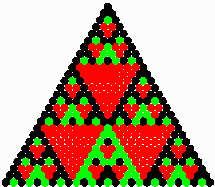
\includegraphics[width=2in]{online-competition-2021-03-04/pascal-triangle.png}}
\caption{\label{fig:pascal-triangle} Paskāla trijstūris (mod 3).}
\end{figure}

\vspace{10pt}
\begin{problem}
Atrast mazāko naturālo skaitli $n$, kurš var kalpot kā ``pretrunas modulis'', 
pierādot, ka vienādojumam $x^3 + y^3 + z^3 = 1969^2$ nav atrisinājumu veselos skaitļos. 

(T.i. aplūkojot atlikumus, dalot ar $n$, izrādās, ka kreisā puse var dot viena veida atlikumus, 
bet labā puse - citus atlikumus, kas nekad nesakrīt ar kreisās puses atlikumiem.)
\answer{

{\bf Atbilde.} $\mathtt{9}$\\
Izrakstām iespējamās $x^3$ vērtības (mod $m$), kur $m = 2,3,\ldots,9$. 
Moduļus $m = 6$, $m=10$ it kā arī varētu aplūkot (un dažos vienādojumos iegūt pretrunas), 
bet faktiski pretrunas rodas pēc pirmskaitļu (vai pirmskaitļu pakāpju) moduļiem.

{\footnotesize
\[ \left\{ \begin{array}{l}
x^3 \equiv 0,1 \pmod{2}\\
x^3 \equiv 0,1,2 \pmod{3}\\
x^3 \equiv 0,1,3 \pmod{4}\\
x^3 \equiv 0,1,2,3,4 \pmod{5}\\
x^3 \equiv 0,1,6 \equiv 0,1,-1 \pmod{7}\\
x^3 \equiv 0,1,3,5,7 \pmod{8}\\ 
x^3 \equiv 0,1,8 \equiv 0,1,-1 \pmod{9}\\ 
\end{array} \right. \]
}

Ievērojam, ka moduļiem $m=7$ un $m=9$ ir tikai trīs iespējamie atlikumi ($\{ 0,1,-1 \}$).
Vienlaikus labajā pusē ir šādi atlikumi:
\[ \left\{ \begin{array}{l}
1969^2 \equiv 4 \pmod{7}\\
1969^2 \equiv 4 \pmod{9}\\
\end{array} \right. \]
Vērtībai $m=7$ atlikumu $4$ var iegūt saskaitot $-1$ trīs reizes: $(-1) + (-1) + (-1) \equiv 4 \pmod{7}$.
Arī pie $m<7$ pretrunas modulis nesanāk, jo kubu summa pieņem jebkādas vērtības.

Atliek pretrunas modulis $m=9$, kas arī ir mūsu atbilde.
}
\end{problem}

\vspace{20pt}
\begin{problem}
Dots kongruenču vienādojums $x^{16} \equiv a \pmod{13}$.
Cik dažādām vērtībām $a$ no kopas $\{0,1,2,\ldots,12\}$ eksistē atrisinājums $x$? 
\answer{

{\bf Atbilde.} $\mathtt{4}$. 

Ja $x \equiv 0 \pmod{13}$, tad $x^{16} \equiv 0 \pmod{13}$. 
Visiem $x \not\equiv 0$ izpildās Mazā Fermā teorēma pirmskaitlim $p=13$: $x^{12} \equiv 1 \pmod{13}.$
Tāpēc $x^{16} \equiv x^{12} \cdot x^{4} \equiv x^{4} \pmod{13}$. 

Kāpināsim visus atlikumus $\{ 1,2,3,4,5,6,7,8,9,10,11,12 \}$ ceturtajā pakāpē. 
Ņemot vērā to, ka $12 \equiv -1 \pmod{13}$, $11 \equiv -2 \pmod{13}$, utt. \textendash{}
pietiek kāpināt ceturtajā (pāru) pakāpē tikai pirmos sešus. 
Iegūstam vērtības $1,3,9$.
Kopā ar atlikumu $0$ ir četras iespējamās $a$ vērtības: $\{0,1,3,9 \}$.

{\footnotesize
{\em Piezīme.} Diezgan jauki vērot, kā mainās dažādo iespējamo $a$ vērtību skaits 
atkarībā no kāpinātāja $k$ kongruencē $x^k \equiv a$ (izņemot vērtību $a \equiv 0$, 
kam vienmēr atbilst $x \equiv 0$). 
Apkoposim tabulā dažādo $a \not\equiv 0$ vērtību skaitu, kurām vienādojumu $x^k \equiv a \pmod{13}$ var atrisināt.

\begin{tabular}{|l|l|r|} \hline
$k$ & $a$ vērtības & Kopskaits \\ \hline
$1$ & $\{ 1,2,3,4,5,6,7,8,9,10,11,12 \}$ & $12$ \\ \hline
$2$ & $\{ 1, 3, 4, 9, 10, 12 \}$ & $6$ \\ \hline
$3$ & $\{ 1, 5, 8, 12 \}$ & $4$ \\ \hline
$4$ & $\{ 1, 3, 9 \}$ & $3$ \\ \hline
$5$ & $\{ 1,2,3,4,5,6,7,8,9,10,11,12 \}$ & 12 \\ \hline
$6$ & $\{ 1,12 \}$ & 2\\ \hline
$7$ & $\{ 1,2,3,4,5,6,7,8,9,10,11,12 \}$ & $12$ \\ \hline
$8$ & $\{ 1, 3, 9 \}$ & $3$ \\ \hline
$9$ & $\{ 1, 5, 8, 12 \}$ & $4$ \\ \hline
$10$ & $\{ 1, 3, 4, 9, 10, 12 \}$ & $6$ \\ \hline
$11$ & $\{ 1,2,3,4,5,6,7,8,9,10,11,12 \}$ & $12$ \\ \hline
$12$ & $\{ 1 \}$ (Mazā Fermā teorēma) & $1$ \\ \hline\hline
$13$ & $\{ 1,2,3,4,5,6,7,8,9,10,11,12 \}$ & $12$ \\ \hline
$14$ & $\{ 1, 3, 4, 9, 10, 12 \}$ & $6$ \\ \hline
$15$ & $\{ 1, 5, 8, 12 \}$ & $4$ \\ \hline
$16$ & $\{ 1, 3, 9 \}$ & $3$ \\ \hline
\end{tabular}

Dažādo nenulles kongruenču klašu skaitu priekš $x^k$ var iegūt ar vienkāršu formulu: ${\displaystyle \frac{12}{\text{LKD}(12,k)}}$
jeb vispārīgā gadījumā ja (mod $p$) ir patvaļīgs pirmskaitlis: ${\displaystyle \frac{p-1}{\text{LKD}(p-1,k)}}$.
}
}
\end{problem}




\end{document}









